\documentclass[border=4pt]{standalone}
\usepackage{amsmath,amssymb}
\usepackage{tikz}
\usetikzlibrary{arrows.meta,calc,decorations.pathreplacing,patterns,shapes.geometric,positioning,shadings,plotmarks}

\begin{document}
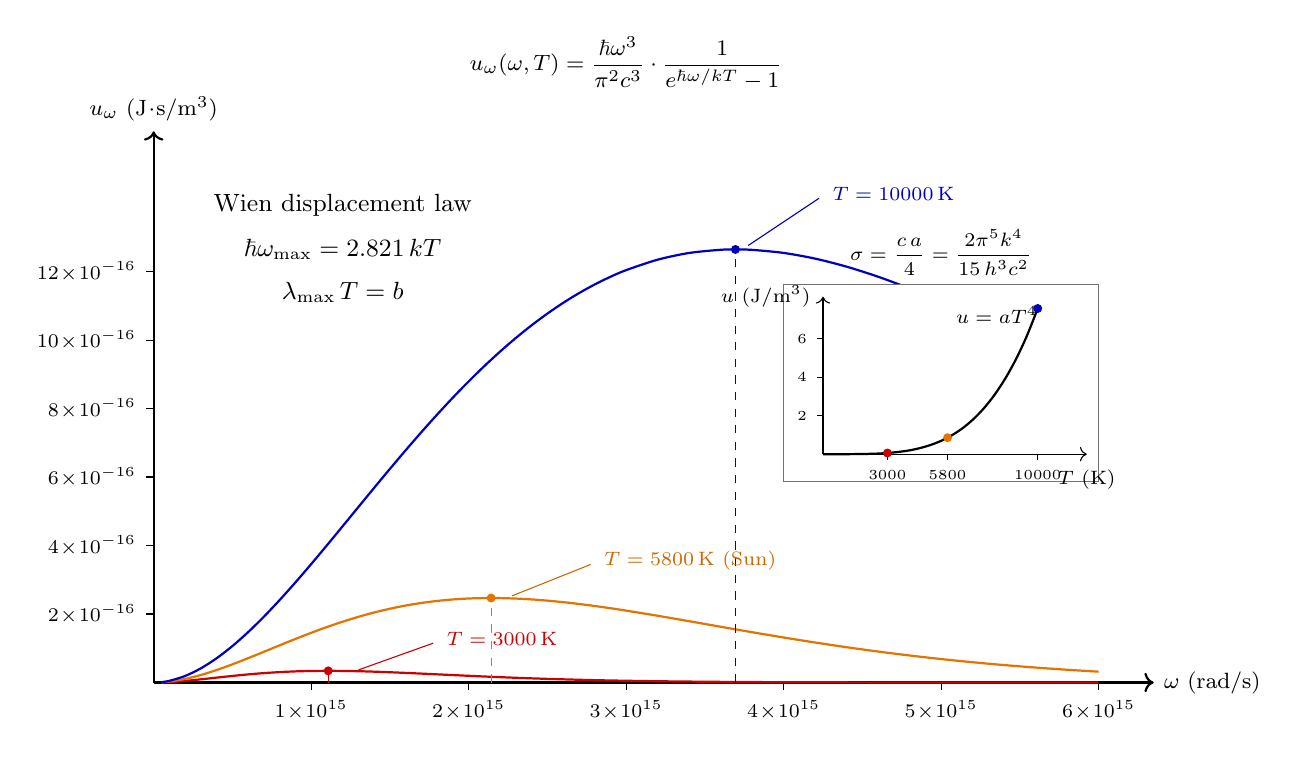
\begin{tikzpicture}[
  every node/.style={font=\footnotesize}
]

% =====================================================================
% Constants (SI):
%   hbar = 1.0546e-34 J*s,  k = 1.381e-23 J/K,  c = 2.998e8 m/s
%   x_max (Wien) = 2.821 -> hbar*omega_max = 2.821 k T
%   omega_max(T):
%     T=3000  K -> 1.108e15 rad/s
%     T=5800  K -> 2.143e15 rad/s
%     T=10000 K -> 3.694e15 rad/s
%
% Plot scaling (main panel):
%   x-axis: omega in [0, 6e15] rad/s -> 12 cm  (xS = 2.0 cm/(1e15 rad/s))
%   y-axis: u_omega scaled so 10000 K peak (1.265e-15 J*s/m^3) -> y=5.5 cm
%           yS = 4.349e15 cm/(J*s/m^3)  -> 5800K peak ~1.07 cm, 3000K peak ~0.15 cm
%   Coordinates below were precomputed from u_omega(omega,T) numerically,
%   so the .tex file does not call exp() in pgfmath (avoids overflow).
% =====================================================================

% --- Top label: Planck formula ---
\node[anchor=south] at (6.0,7.4)
  {$u_\omega(\omega,T) = \dfrac{\hbar\omega^3}{\pi^2 c^3}\cdot\dfrac{1}{e^{\hbar\omega/kT}-1}$};

% --- Axes ---
\draw[->,thick] (0,0) -- (12.7,0) node[right] {$\omega\ (\mathrm{rad/s})$};
\draw[->,thick] (0,0) -- (0,7.0) node[above] {$u_\omega\ (\mathrm{J\!\cdot\!s/m^3})$};

% X ticks at 1, 2, 3, 4, 5, 6 (in 10^15 rad/s)
\foreach \xv in {1,2,3,4,5,6} {
    \pgfmathsetmacro{\xc}{2.0*\xv}
    \draw (\xc,0) -- (\xc,-0.10);
    \node[below] at (\xc,-0.10) {\scriptsize $\xv\!\times\!10^{15}$};
}

% Y ticks at 2,4,6,8,10,12 (in 10^-16 J*s/m^3)
\foreach \yv/\yc in {2/0.870,4/1.740,6/2.610,8/3.480,10/4.349,12/5.219} {
    \draw (0,\yc) -- (-0.10,\yc);
    \node[left] at (-0.10,\yc) {\scriptsize $\yv\!\times\!10^{-16}$};
}

% =====================================================================
% T = 3000 K (red, low temperature)
%   omega_max = 1.108e15 rad/s   peak height ~0.149 cm
% =====================================================================
\draw[red!80!black,thick,smooth] plot coordinates {
    (0.100,0.0016) (0.200,0.0059) (0.400,0.0208) (0.600,0.0406)
    (0.800,0.0624) (1.000,0.0838) (1.200,0.1033) (1.400,0.1196)
    (1.600,0.1324) (1.800,0.1414) (2.000,0.1467) (2.216,0.1485)
    (2.400,0.1473) (2.600,0.1436) (2.800,0.1379) (3.000,0.1306)
    (3.200,0.1222) (3.400,0.1132) (3.600,0.1039) (3.800,0.0945)
    (4.000,0.0853) (4.200,0.0764) (4.400,0.0681) (4.600,0.0602)
    (4.800,0.0530) (5.000,0.0464) (5.400,0.0351) (5.800,0.0261)
    (6.400,0.0164) (7.200,0.0084) (8.000,0.0042) (9.000,0.0018)
    (10.000,0.0006) (12.000,0.0001)
};
\draw[red!80!black,dashed,thin] (2.216,0) -- (2.216,0.1485);
\filldraw[red!80!black] (2.216,0.1485) circle (1.4pt);

% =====================================================================
% T = 5800 K (orange/yellow, sun)
%   omega_max = 2.143e15 rad/s   peak height ~1.073 cm
% =====================================================================
\draw[orange!90!black,thick,smooth] plot coordinates {
    (0.100,0.0032) (0.200,0.0123) (0.400,0.0458) (0.600,0.0961)
    (0.800,0.1591) (1.000,0.2313) (1.200,0.3094) (1.400,0.3907)
    (1.600,0.4727) (1.800,0.5534) (2.000,0.6312) (2.200,0.7046)
    (2.400,0.7726) (2.600,0.8344) (2.800,0.8894) (3.000,0.9372)
    (3.200,0.9777) (3.400,1.0107) (3.600,1.0365) (3.800,1.0551)
    (4.000,1.0671) (4.200,1.0726) (4.285,1.0731) (4.400,1.0722)
    (4.600,1.0663) (4.800,1.0554) (5.000,1.0400) (5.200,1.0207)
    (5.400,0.9978) (5.600,0.9720) (5.800,0.9437) (6.000,0.9133)
    (6.400,0.8479) (6.800,0.7788) (7.200,0.7085) (7.600,0.6390)
    (8.000,0.5719) (8.400,0.5081) (8.800,0.4485) (9.200,0.3935)
    (9.600,0.3434) (10.000,0.2982) (10.400,0.2576) (10.800,0.2217)
    (11.200,0.1899) (11.600,0.1621) (12.000,0.1379)
};
\draw[orange!90!black,dashed,thin] (4.285,0) -- (4.285,1.0731);
\filldraw[orange!90!black] (4.285,1.0731) circle (1.4pt);

% =====================================================================
% T = 10000 K (blue, high temperature)
%   omega_max = 3.694e15 rad/s   peak height ~5.500 cm
% =====================================================================
\draw[blue!75!black,thick,smooth] plot coordinates {
    (0.100,0.0055) (0.200,0.0217) (0.400,0.0836) (0.600,0.1808)
    (0.800,0.3088) (1.000,0.4634) (1.200,0.6406) (1.400,0.8367)
    (1.600,1.0481) (1.800,1.2715) (2.000,1.5040) (2.200,1.7429)
    (2.400,1.9855) (2.600,2.2294) (2.800,2.4727) (3.000,2.7134)
    (3.200,2.9498) (3.400,3.1803) (3.600,3.4036) (3.800,3.6185)
    (4.000,3.8241) (4.200,4.0194) (4.400,4.2037) (4.600,4.3765)
    (4.800,4.5372) (5.000,4.6856) (5.200,4.8214) (5.400,4.9445)
    (5.600,5.0548) (5.800,5.1524) (6.000,5.2373) (6.400,5.3701)
    (6.800,5.4553) (7.200,5.4957) (7.388,5.5001) (7.600,5.4946)
    (8.000,5.4558) (8.400,5.3834) (8.800,5.2812) (9.200,5.1535)
    (9.600,5.0040) (10.000,4.8367) (10.400,4.6551) (10.800,4.4624)
    (11.200,4.2619) (11.600,4.0561) (12.000,3.8476)
};
\draw[blue!75!black,dashed,thin] (7.388,0) -- (7.388,5.5001);
\filldraw[blue!75!black] (7.388,5.5001) circle (1.4pt);

% Curve labels with leader lines
\node[red!80!black,anchor=west] at (3.6,0.55) {\scriptsize $T=3000\,\mathrm{K}$};
\draw[red!80!black,thin] (3.55,0.50) -- (2.6,0.16);

\node[orange!80!black,anchor=west] at (5.6,1.55) {\scriptsize $T=5800\,\mathrm{K}\ (\mathrm{Sun})$};
\draw[orange!80!black,thin] (5.55,1.50) -- (4.55,1.10);

\node[blue!75!black,anchor=west] at (8.5,6.20) {\scriptsize $T=10000\,\mathrm{K}$};
\draw[blue!75!black,thin] (8.45,6.15) -- (7.55,5.55);

% Wien displacement annotation
\node[anchor=south,align=center] at (2.4,5.8)
  {\small Wien displacement law};
\node[anchor=south,align=center] at (2.4,5.25)
  {\small $\hbar\omega_{\max} = 2.821\, kT$};
\node[anchor=south,align=center] at (2.4,4.70)
  {\small $\lambda_{\max}\, T = b$};

% =====================================================================
% INSET (top right): u(T) = a T^4 with three temperatures marked.
% Inset frame: 4 cm wide, 2.4 cm tall, anchored at xshift=8.0, yshift=2.6
% Inside the inset, axes start at (0.45, 0.30); usable area ~3.35 x 1.95.
% =====================================================================
\begin{scope}[xshift=8.05cm,yshift=2.60cm]

% Inset frame
\draw[fill=white,draw=black!55,line width=0.4pt] (-0.05,-0.05) rectangle (3.95,2.45);

% Inset axes
\draw[->,thin] (0.45,0.30) -- (3.80,0.30) node[below=2pt,font=\scriptsize] {$T\ (\mathrm{K})$};
\draw[->,thin] (0.45,0.30) -- (0.45,2.30) node[left=1pt,font=\scriptsize] {$u\ (\mathrm{J/m^3})$};

% T-axis ticks at 3000, 5800, 10000.  T-axis spans 0..11000 over 3.0 cm.
%   xT(T) = 0.45 + 3.0*T/11000
\foreach \tv/\xv in {3000/1.268,5800/2.032,10000/3.177} {
    \draw[thin] (\xv,0.30) -- (\xv,0.22);
}
\node[font=\tiny,below] at (1.268,0.22) {$3000$};
\node[font=\tiny,below] at (2.032,0.22) {$5800$};
\node[font=\tiny,below] at (3.177,0.22) {$10000$};

% u-axis ticks at u=2, 4, 6 (J/m^3): yT(u) = 0.30 + 1.85*u/7.566
\foreach \uv/\yv in {2/0.789,4/1.278,6/1.767} {
    \draw[thin] (0.45,\yv) -- (0.37,\yv);
    \node[font=\tiny,left] at (0.37,\yv) {$\uv$};
}

% u = a T^4 curve, sampled.  Coords precomputed: x = 0.45+3.0*T/11000, y = 0.30+1.85*u/7.566
\draw[black,thick,smooth] plot coordinates {
    (0.450,0.300) (0.586,0.300) (0.723,0.300) (0.859,0.301)
    (0.995,0.303) (1.132,0.307) (1.268,0.315) (1.405,0.328)
    (1.541,0.347) (1.677,0.376) (1.814,0.416) (1.950,0.469)
    (2.086,0.540) (2.223,0.630) (2.359,0.744) (2.495,0.885)
    (2.632,1.058) (2.768,1.266) (2.905,1.514) (3.041,1.807)
    (3.177,2.150)
};

% Three data points
\filldraw[red!80!black] (1.268,0.315) circle (1.4pt);
\filldraw[orange!90!black] (2.032,0.509) circle (1.4pt);
\filldraw[blue!75!black] (3.177,2.150) circle (1.4pt);

% Inset curve label
\node[anchor=north east,font=\scriptsize] at (3.30,2.30) {$u = a T^4$};

% Sigma formula above the inset frame
\node[anchor=south,font=\scriptsize] at (1.95,2.45)
  {$\sigma = \dfrac{c\, a}{4} = \dfrac{2\pi^5 k^4}{15\, h^3 c^2}$};

\end{scope}

\end{tikzpicture}
\end{document}
